\subsection{\textsf{PacMan}: A \DSL for the PacMan game}
\label{sec:Examples:PacMan}

The PacMan game is a popular arcade game that gained interest in the \MDE community
because it captures a well-known, simple reactive \DSL with an easily understandable
concrete syntax, and presents interesting real-time features for execution. 

\subsubsection{Specification}
\label{sec:Examples:PacMan:Specification}

On the top left compartment is represented a metamodel
$\mathsf{MM}_{\mathsf{PM}}$, as created by a DSL engineer. A \textsf{Game} 
consists of a sequence of \textsf{Level}s, each displaying a \textsf{Maze} where
\textsf{Persona}s evolve. A \textsf{Level} terminates when \textsf{PacMan} is eaten
by a \textsf{Ghost}, or when it has eaten all \textsf{Cookie}s. Several players
may compete for the highest \textsf{Score}.

On the top right compartment, a basic model $\mathsf{M}_{\mathsf{2x2}}$ with a
\textsf{unique} \textsf{Level} of size 2x2, as possibly created by a modeller,
is depicted using three different concrete syntaxes:
textual for $^{\mathsf{TXT}}\mathsf{M}_{\mathsf{2x2}}$ (inspired by eMotions 
\cite{J:RiveraDuranVallecillo:2009}); based on UML Object Diagram for
\cite{B:Rumbaugh-Jacobson-Booch:2004} for $^{\mathsf{OD}}\mathsf{M}_{\mathsf{2x2}}$;
and freely inspired by the real game for $^{\mathsf{Viz}}\mathsf{M}_{\mathsf{2x2}}$,
the two latters being graphical.

\begin{figure*}[t]
   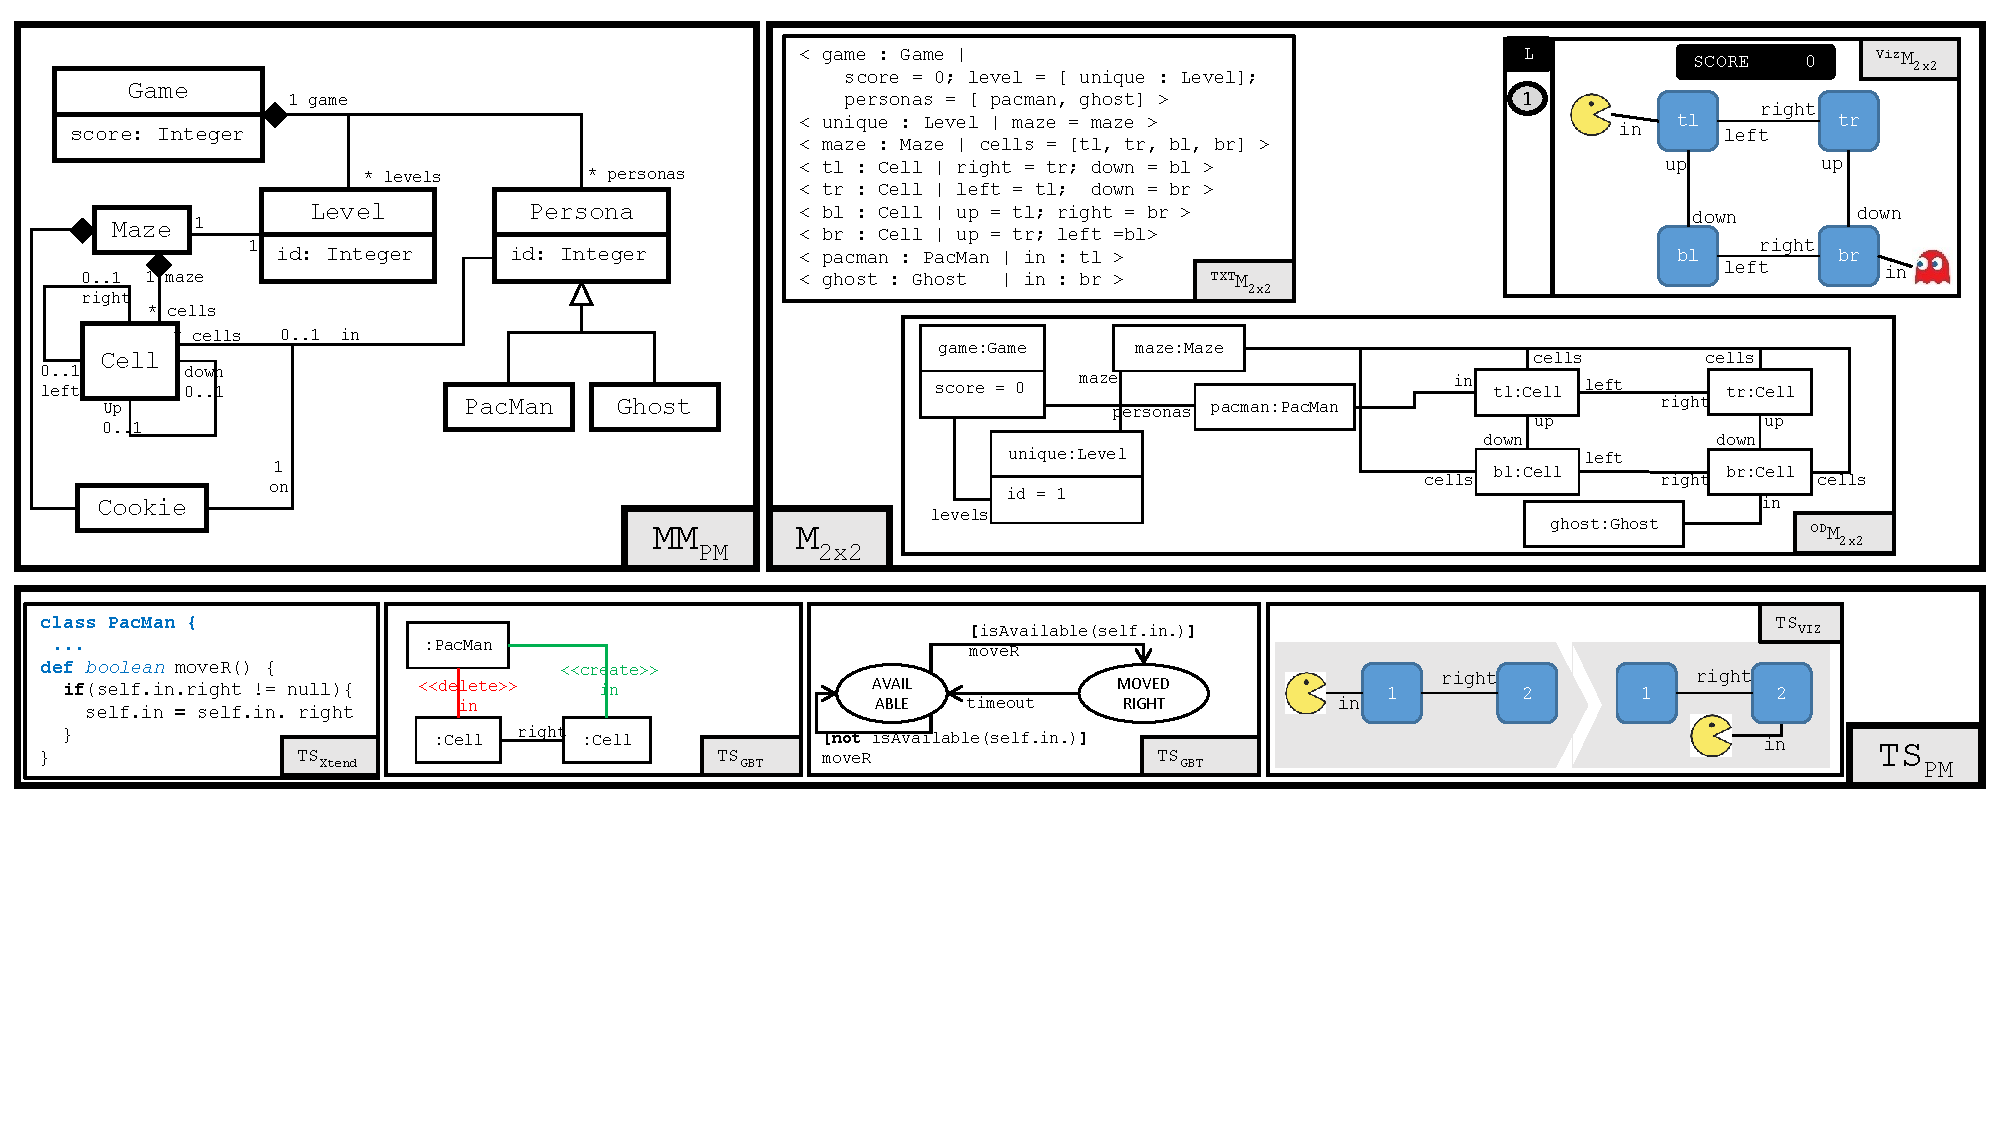
\includegraphics[width=\textwidth,clip, trim=0cm 5.5cm 0cm 0cm]{MM-M-T.pdf}
   \caption{Specifying a Pac-Man DSL: the DSL engineer create the metamodel 
   $\mathsf{MM}_{\mathsf{PM}}$; a modeller chooses a concrete syntax to create
   a simple model $\mathsf{M}_{\mathsf{2x2}}$; a MT designer specifies a transformation
   $\mathsf{TS}_{\mathsf{PM}}$ (only the \emph{\textsf{moveR}} MT unit is shown).%
   \MA{Introduce notation for DDM/SDM!}}
   \label{fig:PacMan}
   \Description[<short description>]{<long description>}
\end{figure*}

\subsubsection{Execution}
\label{sec:Examples:PacMan:Execution}

The bottom compartment of \autoref{fig:PacMan} describes a simple rule 
\emph{\textsf{moveR}} (moving Pac-Man on a \textsf{Cell} at its right, if 
available) as part of the simulation MT specification $\mathsf{TS}_{\mathsf{PM}}$,
as part of $\mathsf{MM}_{\mathsf{PM}}$'s executable semantics. 
The first MT, $\mathsf{TS}_{\mathsf{Xtend}}$, uses metaprogramming 
(based on Xtend with GeMoC \cite{Leroy-Bousse-etAl:2017}). The next and last ones
are based on Graph Transformations: $\mathsf{TS}_{\mathsf{GBT}}$ relies on 
$^{\mathsf{OD}}\mathsf{M}_{\mathsf{2x2}}$ to express the rewriting (as would be 
expressed e.g. in Henshin \cite{Bill-Gabmeyer-Kaufmann-Seidl:2014}); 
while $\mathsf{TS}_{\mathsf{VIZ}}$ relies on $^{\mathsf{Viz}}\mathsf{M}_{\mathsf{2x2}}$
(as would be expressed e.g. in AtoMPM \cite{J:SyrianiVangheluwe:2013}). 
Finally, $\mathsf{TS}_{\mathsf{FSM}}$ presents an MT fragment expressed with 
a UML's Finite State Machine \cite{B:Rumbaugh-Jacobson-Booch:2004}. 
Note that all MT specifications (fragments) but $\mathsf{TS}_{\mathsf{Xtend}}$ 
present a graphical representation, showing that MT specifications may well be 
graphically visualised as well.

\subsubsection{Animations}
\label{sec:Examples:PacMan:Animations}

The PacMan game typically uses three kinds of animations for different situations:
\begin{description}
   \item[A \textsf{Persona} moves.] Typically, a specific animation could be attached
   to each movement, as they are traditionally encoded in different rules/operations
   (cf. e.g. \textsl{moveR} as specified in \autoref{fig:PacMan}, but also 
   \textsl{moveL}, \textsl{moveU} and \textsl{moveD} for moving left, up and down).
   Depending on whether the MTL allows using abstract classes (which would be 
   \textsf{Persona} here) for MT specification, these rules/operations may need 
   to be duplicated. 
   
   \item[\textsf{PacMan} eats a \textsf{Cookie}.] This occurs when \textsf{PacMan} is on a \textsf{Cell}
   that contains a \textsf{Cookie}, making it disappear and triggering a 
   \textsf{Score} update.
   
   \item[\textsf{PacMan} is eaten by a \textsf{Ghost}.] This occurs when 
   \textsf{PacMan} is on the same \textsf{Cell} as a \textsf{Ghost}, which may occur
   by either \textsf{Persona} making a move to an already occupied \textsf{Cell}.
\end{description}
To summarise, we would have to define four different animations to fully animate
the \textsf{PacMan} \DSL:
\begin{description}
   \item[PM.1] The \textsf{Persona} disappears from one \textsf{Cell} and reappears
   on another (adjacent) \textsf{Cell}.
   
   \item[PM.2] Assuming \textsf{PacMan} is on a \textsf{Cell} containing a \textsf{Cookie},
   the \textsf{Cookie} disappears.
   
   \item[PM.3] The \textsf{Score} is updated by a given increment. 

   \item[PM.4] Assuming \textsf{PacMan} and a \textsf{Ghost} are on the same
   \textsf{Cell}, \textsf{PacMan} disappears.
\end{description}
Note that those animations are not completely unrelated. First, \textbf{PM.2} and
\textbf{PM.3} need to be conducted sequentially quickly enough to not notice a
time gap. Second, \textbf{PM.2} and \textbf{PM.4} appear to be very similar in
nature: they both assume that two objects are located on the same \textsf{Cell} 
before making one of them disappear.

